\documentclass{scrartcl}
\usepackage[utf8]{inputenc}
\usepackage{graphicx}
\title{Project: Power Cloud}
\subtitle{Client: Hanrich Potgieter \\ Team: Quadcore Productions\\}
\author{Themba Mbhele 14007950\\ Moses Mayimela 14019702 \\ Hlengekile Jita 14077893 \\ Mpho Baloyi 14133670 \\Department of Computer Science, University of Pretoria}
\date{01 May 2016}


\begin{document}

\maketitle
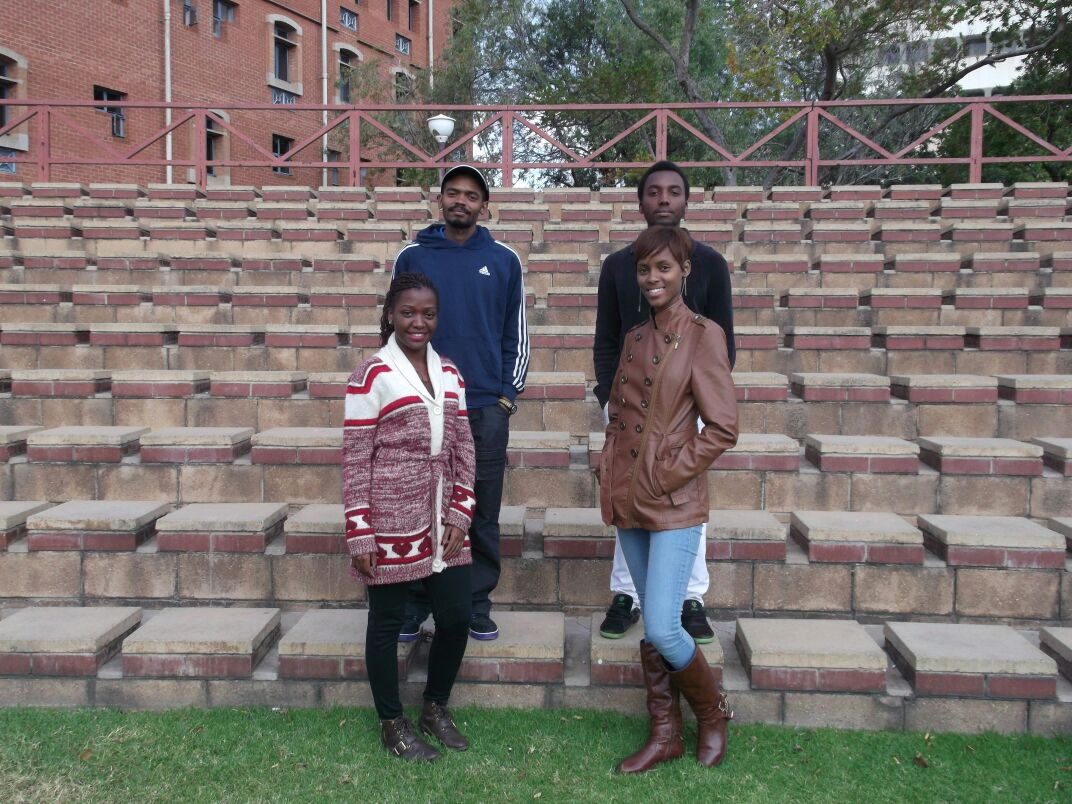
\includegraphics[width=\textwidth]{images/GroupPhoto}
\section{The Team}
\subsection{Mpho Baloyi}
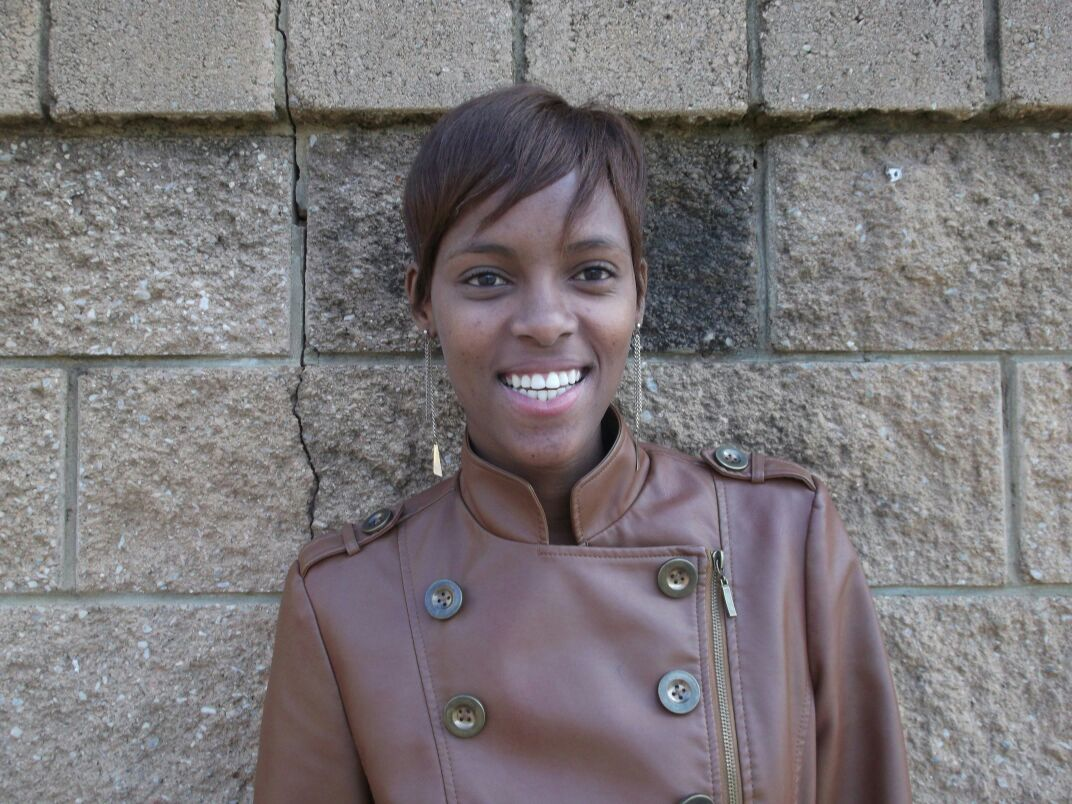
\includegraphics[width=\textwidth]{images/Mpho}
\subsubsection{Interests}
\begin{itemize}
\item Keeping abreast with new technologies
\item Learning and using new technologies to solve problems
\item Reading up and doing research on new and old concepts in computer science
\item Solving riddles and puzzles
\item Helping people through ICT
\end{itemize}
\subsubsection{Technical Skills}
\begin{itemize}
\item Solid programming skills in java,c++ and python
\item Fair amount of knowlegde in assembly programming
\item Web development with HTML,JAVASCRIPT,JQUERY,CSS,PHP,AJAX,ANGULARJS
\item Interaction Design
\item Database design with MySQL
\item Understanding of process development
\item Unit testing,mocking and dependency Injection
\end{itemize}
\subsubsection{Non-Technical Strengths}
\begin{itemize}
\item Excellent Communication skills
\item Patient
\item Creative approach to problem solving
\item Pay attention to detail
\item Excellent planning skills
\item Ability to grasp concepts quickly
\item Willness to learn new things
\item Ability to interpret and follow technical plans
\item Ability to collaborate and work efficiently with other people
\item Ability to work under pressure
\end{itemize}
\subsubsection{Relevant Past Experiences}
Work in the mini-project of the university of Pretoria taught me impoortant skills in software engineering such as unit testing,dependency injection,mocking and working with different technologies. I believe that these skills will be valuable to the development of this project as they apply in every area of software development.
\subsubsection{Reasons for wanting to do the project}
I want to do this project because it provides me with the opportunity to work with different kinds of technologies and devices and to learn new ways of collecting data.
\newpage
\subsection{Hlengekile Jita}
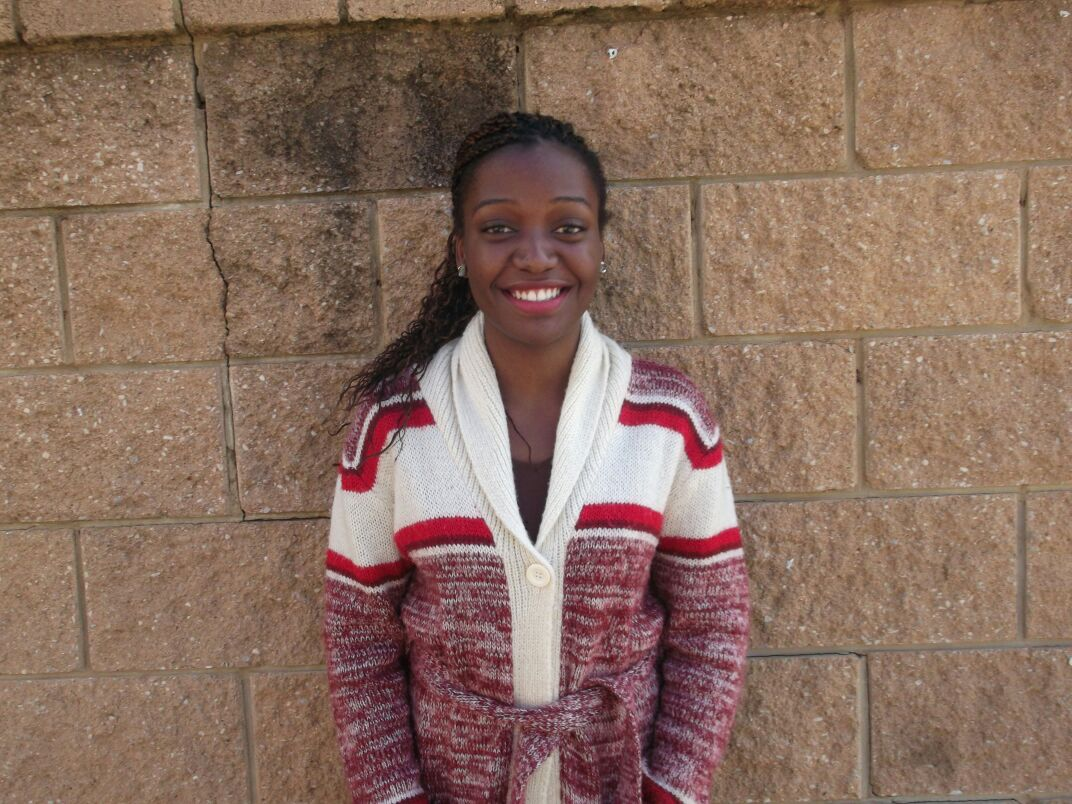
\includegraphics[width=\textwidth]{images/Hlengi}
\subsubsection{Interests}
\subsubsection{Technical Skills}
\begin{itemize}
\item Microsoft Office - Word, Excel, Access, PowerPoint
\item Programming - Java, C++, Python, Android
\item Database Design - MySQL
\item Web Development - XHTML, HTML5, CSS, JavaScript, PHP
\end{itemize}
\subsubsection{Non-Technical Strengths}
\begin{itemize}
\item Good leader
\item Excellent communication skills both verbal and written
\item Works well under pressure
\item Great at teamwork
\item Sociable character that gets along with people
\item Organized individual with meticulous planning skills
\item Determined
\end{itemize}
\subsubsection{Relevant Past Experiences}
\subsubsection{Reasons for wanting to do the project}
\newpage
\subsection{Moses Mayimela}
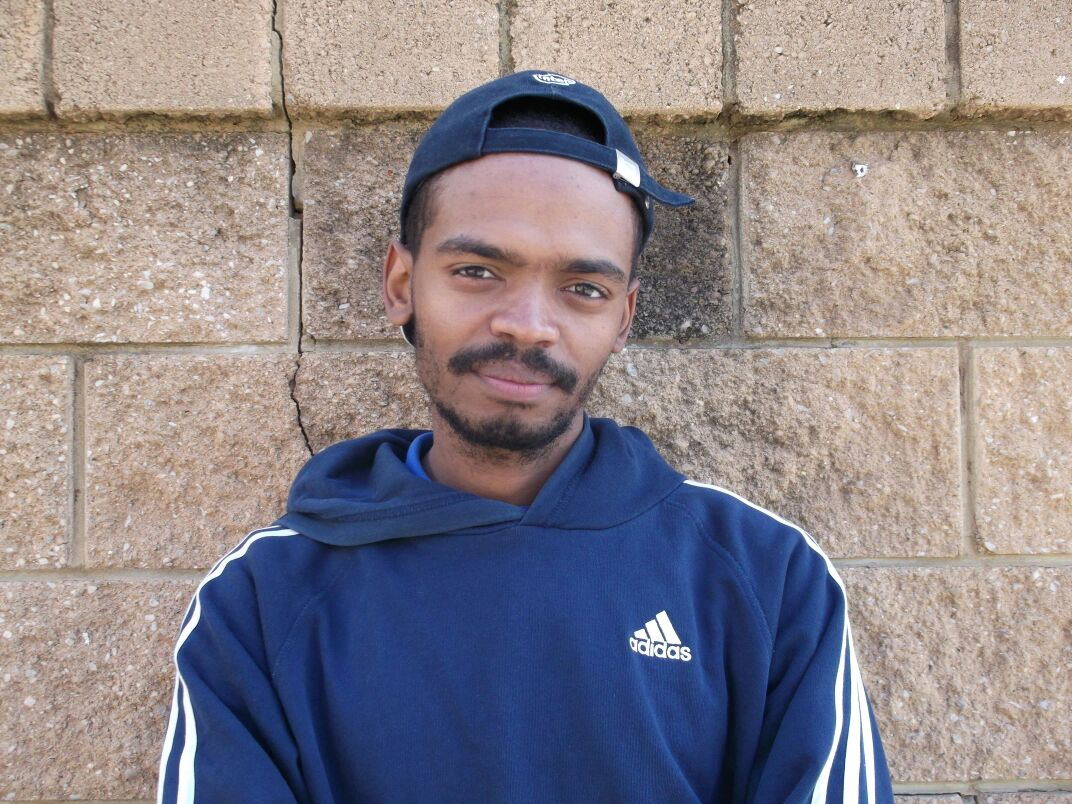
\includegraphics[width=\textwidth]{images/Moses}
\subsubsection{Interests}
\begin{itemize}
\item Keeping up to date with the latest technologies e.g Raspberry pi and Intel Edison.
\item Reading Tech reviews and comparisons on software and hardware systems such as BLE vs Classic bluetooth.
\item Taking part in hackerthons e.g Hack4Water.
\end{itemize}
\subsubsection{Technical Skills}
\begin{itemize}
\item Programming skills in:
\begin{enumerate}
\item Java.
\item C for embedded Systems (8 bit and 32 bit) and PC applications.
\item C++.
\item C\#.
\item Python.
\end{enumerate}
\item knowlegde in assembly programming for embedded (8 bit and 32 bit) and PC applications.
\item Web development with:\\
HTML,CSS, Javascript, NodeJS (Javascript framework),PHP and AJAX
\item Database design with MySQL,MSSQL and Postgresql.
\item Unit testing,mocking and dependency Injection
\item Familiar with GSM/3G Modules AT commands.
\item Experience with Linux servers.
\end{itemize}
\subsubsection{Non-Technical Strengths}
\begin{itemize}
\item I like working with people who love what they do.
\item I can lead a team and I also respect a leader.
\item I am always willing to learn and expand my horizons.
\item I am open minded to people's opinions.
\end{itemize}
\subsubsection{Relevant Past Experiences}
\begin{itemize}
\item Won, breakthrough developer award for 2015 in the MTN M2M (IoT) competition.\\
http://www.mind2machine.co.za \\
https://www.youtube.com/watch?v=HZlryrw1Ois.
\item 2nd place at the Hack4Water Hackathon in April 2016.\\
https://twitter.com/hashtag/hack4water
\end{itemize}
\subsubsection{Reasons for wanting to do the project}
This project will provide an opportunity for me to expand my knowledge in programming while providing a fully functional solution for the client. The technologies in this project will also help me learn better software standards. Through this project, I can personally learn how I can make myself better and improve my contribution in a way that matters when working with people.
\newpage
\subsection{Themba Mbhele}
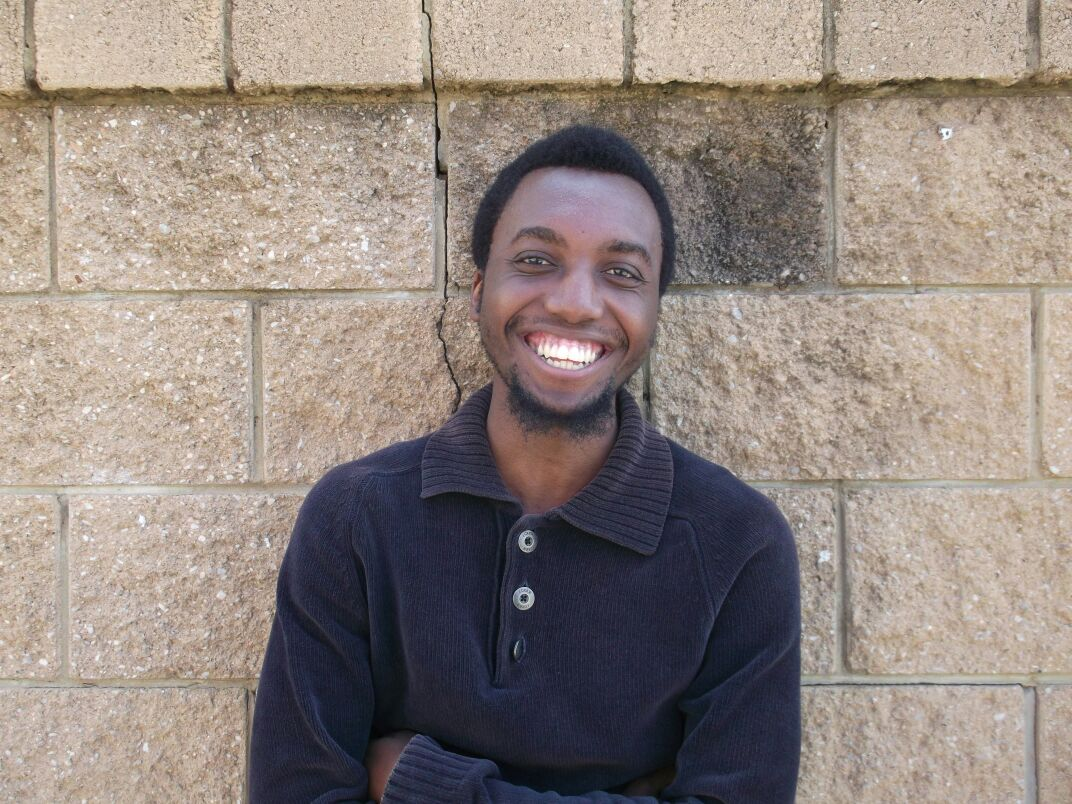
\includegraphics[width=\textwidth]{images/Themba}
\subsubsection{Interests}
\begin{itemize}
    \item Gaming
    \item Artificial Intelligence
    \item New developments in the Computer Science field
    \item Basketball
\end{itemize}
\subsubsection{Technical Skills}
\begin{itemize}
    \item Strong programming skills in C++ and Java
    \item Web Dev - HTML5, CSS, WebGL, JavaScript, PHP
\end{itemize}
\subsubsection{Non-Technical Strengths}
\begin{itemize}
    \item Excellent time management skills
    \item Dedicated student
    \item Team player
\end{itemize}
\subsubsection{Reasons for wanting to do the project}
I believe that performance analysis is key not only to businesses, but also on a personal level. I want to be a part of this project so that I can learn what are the key performance measures that determine how optimal an 
individual or team is so that I may know which techniques or tactics should be used to improve efficiency.
\newpage
\section{Project Execution}
\subsection{Development Methodology}
\subsection{Communication With Client}
To keep the clients informed we are going to use the following means of communication
\subsubsection{email}
\begin{itemize}
\item To inform the client of our progress
\item To address any issues or concerns that they client may have
\item To acquire information from the client
\item To require any resources that the client has to offer for their project,..
\end{itemize}

\subsubsection{Phone calls}
 This will only be used to address very urgent matters if they arise during the course of the project development 
 however this will only be done with permission from the client and during business hours.
 
\subsubsection{Regular Meetings}	 
These will take place depending on the clients availiability and willness.
We may discuss the progress of the project,to address any concerns,etc.

\subsubsection{GIT}

Access to our git repository will be provided to the client,so the client can be able to monitor
our progress and have access to the project material.

We are also open to any means of communicatiuon that the client may prefer or suggest.

\subsection{Technical Challenges}
\subsection{Technologies}
This section will list the technologies that will be used to implement the system.\\
To implement the back-end of the system, the following technologies will be used:
\begin{itemize}
    \item NodeJS will be used to implement the server.
    \item MongoDB will be used to store the data that will be collected.
    \item C++ will be used to program the hardware
\end{itemize}
To implement the front-end of the system, the following technologies will be used:
\begin{itemize}
    \item AngularJS will be used for the web front-end.
\end{itemize}

\end{document}
